\chapter{Buchi neri}
In questo capitolo verranno investigate maggiormente le proprietà dei buchi neri, in particolar modo le proprietà dell'orizzonte per poi trattare il legame con la termodinamica e la radiazione di Hawking. Si farà infine un accenno ad buco nero di Banados-Teitelboim-Zanelli.
\section{Ipersuperfici nulle e gravità superficiale}
\begin{definizione}
Sia $S(x)$ una funzione liscia sullo spaziotempo di coordinate $x^\mu$ e si considerino la famiglia di ipersuperfici $S = \textrm{cost.}$. I \textbf{campi vettoriali normali all'ipersuperficie} sono definiti da:
\begin{equation}
    l = \Tilde{f}(x)(g^{\mu\nu}\partial_\nu S) \frac{\partial}{\partial x^\mu}
    \label{eq.vettore_normale_ipersup}
\end{equation}
per una qualche funzione non nulla $\Tilde{f}$. Se $l^2 = 0$ per una qualche ipersuperficie $N$ nella famiglia, allora $N$ è una \textbf{ipersuperficie nulla}.
\end{definizione}
Tra le varie ipersuperfici nulle di nostro interesse, c'è l'orizzonte degli eventi. Vediamo quindi le loro proprietà.

Sia $N$ un'ipersuperficie nulla con $l$ vettore normale e sia $\phi$ un vettore tangente a $N$, ovvero $<\phi, l> = 0$.  Siccome $l$ è un vettore nullo, $<l,l> = 0$ allora $l$ è anche un vettore tangente. Pertanto in un'ipersuperficie nulla i \textbf{vettori normali sono anche tangenti}. Essendo un vettore tangente, esisterà la sua curva integrale (nulla) $x^\mu$ in $N$ tale che $l^\mu = \frac{dx^\mu}{d\lambda}$, rispetto $\lambda$ parametro della curva.
Per queste curve nulle sull'ipersuperficie nulla si ha il lemma:
\begin{lemma}
Le curve $x^\mu$ sono geodetiche.
\end{lemma}
\begin{proof}
Sia $N$ il membro $S=0$ della famiglia (non necessariamente nulla) di ipersuperfici $S(x^\mu) = \textrm{cost.}$
Consideriamo la scrittura di $l^\mu$ di eq.\ref{eq.vettore_normale_ipersup}. Per verificare sia una geodetica, calcoliamo la derivata covariante lungo $l$ del vettore stesso:
\begin{align}
    \nabla_l l^\mu &= l^\rho \nabla_\rho l^\mu =  l^\rho \nabla_\rho (\Tilde{f}(x)g^{\mu\nu}\partial_\nu S ) = (l^\rho \partial_\rho \Tilde{f}) g^{\mu\nu}\partial_\nu S + \Tilde{f}g^{\mu\nu}l^\rho \nabla_\rho \partial_\nu S \nonumber \\
    &= \left(\frac{dx^\rho}{d\lambda} \partial_\rho \Tilde{f} \right) \frac{l^\mu}{\Tilde{f}} + \Tilde{f}g^{\mu\nu}l^\rho (\partial_\rho\partial_\nu S - \tensor{\Gamma}{^\lambda_{\rho\nu}}\partial_\lambda S)  \nonumber\\
    &= \left(\frac{dx^\rho}{d\lambda}\partial_\rho\log\Tilde{f}\right)l^\mu + \Tilde{f}g^{\mu\nu}l^\rho (\partial_\nu\partial_\rho S - \tensor{\Gamma}{^\lambda_{\nu\rho}}\partial_\lambda S) = \left( \frac{d}{d\lambda}\log\Tilde{f}\right)l^\mu + \Tilde{f}g^{\mu\nu}l^\rho \nabla_\nu\partial_\rho S \nonumber \\
    \intertext{Usiamo ora $\partial_\rho S = \Tilde{f}^{-1}g_{\mu\rho}l^\mu$ e la possibilità di portare la metrica entro la derivata covariante:}
    &= \left( \frac{d}{d\lambda}\log\Tilde{f}\right)l^\mu + \Tilde{f}l^\rho \nabla^\mu(\Tilde{f}^{-1}l_\rho) = \left( \frac{d}{d\lambda}\log\Tilde{f}\right)l^\mu + l^\rho \Tilde{f}( \Tilde{f}^{-1}\nabla^\mu l_\rho + \left(\partial^\mu\Tilde{f}^{-1})l_\rho\right) \nonumber \\
    &= \left( \frac{d}{d\lambda}\log\Tilde{f}\right)l^\mu + l^\rho \nabla^\mu l_\rho - (\partial^\mu\log\Tilde{f})l^2 \nonumber \\
    &= \left( \frac{d}{d\lambda}\log\Tilde{f}\right)l^\mu  + \frac{1}{2}\nabla^\mu l^2 - (\partial^\mu \log\Tilde{f})l^2 \label{eq.ipersup_nulla_geodesica}
\end{align}
Il fatto che $l^2=0$ su $N$ non implica necessariamente che $\partial^\mu l^2 =0$ su $N$, a meno che tutta la famiglia di ipersuperfici $S= \textrm{cost.}$ sia nulla. Però se $l^2 = \textrm{cost.}$ su $N$ allora vale che $\phi(l^2) = \phi^\mu \partial_\mu l^2 = 0$ per ogni vettore tangente $\phi$ a $N$. Questo fa sì che:
\begin{equation*}
    \partial_\mu l^2 |_N \propto l_\mu
\end{equation*}
Per il terzo termine si ha semplicemente $(\partial^\mu \log\Tilde{f})l^2 |_N =0$.  Otteniamo dunque che i primi due termini sono proporzionali a $l^\mu$ e allora:
\begin{equation*}
    \nabla_l l^\mu |_N \propto l^\mu
\end{equation*}
che è l'equazione delle geodetiche in parametrizzazione non affine. Poiché $l$ era il vettore tangente di $x^\mu(\lambda)$, questa sarà una curva geodetica.
\end{proof}
Può eventualmente essere scelto un $\Tilde{f}$ così che la parametrizzazione sia affine, $\nabla_l l^\mu =0$.
\begin{definizione}
    Le geodetiche nulle $x^\mu(\lambda)$ con parametro affine $\lambda$ e vettore tangente $\frac{d x^\mu}{d\lambda}$ normale all'ipersuperficie nulla $N$ sono chiamate \textbf{generatori nulli} di $N$.
\end{definizione}

\begin{esempio}
Sia lo spaziotempo di Schwarzschild in coordinate di Kruskal. L'orizzonte futuro $\mathcal{H}^+$ è un'ipersuperficie nulla ottenuta per $U = 0$. In generale la normale all'ipersuperficie $U = \textrm{cost.}$ (diagonali  luce da sinistra a destra nel diagramma di Penrose) è data da:
\begin{equation*}
    l = \Tilde{f}g^{\mu\nu}\partial_\nu S\partial_\mu = \Tilde{f}g^{VU}\partial_{U}S\partial_V = - \frac{\Tilde{f}r}{16m^3}e^{r/2m}\partial_V
\end{equation*}
facendo riferimento alla metrica eq. \ref{eq.metrica_kruskal_UV}. Perciò sull'ipersuperficie nulla, dove $r = 2m$, si ha:
\begin{equation*}
    l|_N = - \frac{\Tilde{f}e}{8m^2}\partial_V
\end{equation*}
In questo caso $l^2 = 0$ poiché $<\partial_V, \partial_V> = 0$ (per ogni costante, $U = \textrm{cost.}$ sono ipersuperfici nulle). Allora si ha anche $\partial_\mu l^2|_N = 0$  come secondo termine di eq. \ref{eq.ipersup_nulla_geodesica}. Otteniamo che la parametrizzazione è affine, $\nabla_l l = 0$, se $\Tilde{f}= \textrm{cost.} $. Possiamo scegliere:
\begin{equation*}
    \Tilde{f}= -\frac{8m^2}{e}
\end{equation*}
così $l = \partial_V$ è vettore normale a $U= 0$. $V$ è un parametro affine per il generatore dell'ipersuperficie nulla.
\end{esempio}

\begin{definizione}
    Un'ipersuperficie nulla $N$ viene chiamata \textbf{orizzonte di Killing} di un campo vettoriale di Killing $\xi$ se $\xi$ è normale a $N$.
\end{definizione}
Sia $l$ normale a $N$ e in parametrizzazione affine. Poiché anche $\xi$ è normale a $N$ si avrà, per qualche funzione $f$  su $N$, $\xi = f l$. Segue che:
\begin{equation*}
    \nabla_\xi \xi = \nabla_{fl}(fl) = f \nabla_l (fl) = f( f\nabla_l l + l(f) l)
\end{equation*}
Su $N$, vale la parametrizzazione affine e allora:
\begin{equation*}
    \nabla_\xi \xi = l(f) \xi =: \kappa \xi
\end{equation*}
dove $\kappa$ viene detta \textbf{gravità superficiale}. In particolare, sviluppando in una base:
\begin{equation}
    \kappa = l(f) = l^\mu \partial_\mu f = f^{-1} \xi^\mu \partial_\mu f = \xi^\mu \partial_\mu \log |f|
    \label{eq.grav_superficiale}
\end{equation}
La gravità superficiale corrisponde all'accelerazione subita da una particella statica vicino all'orizzonte, come misurata da un osservatore posto all'infinito spaziale. La si può pensare come la tensione che avrebbe un filo teso tra un osservatore che sta per varcare l'orizzonte e chi misura, posto all'infinito. Questa interpretazione è meglio chiarita quando si analizza quanto avviene vicino all'orizzonte di accelerazione in uno spaziotempo di Rindler.

Determiniamo ora una formula per $\kappa$ nella quale appare solamente $\xi$. Poiché $\xi$ è normale a $N$ vale il teorema di Frobenius e pertanto:
\begin{equation*}
    \xi_{[\mu}\nabla_{\nu}\xi_{\rho]}|_N = 0 \iff \xi \wedge d\xi
\end{equation*}
Poiché $\xi$ è di Killing, eq. \ref{eq.killing}, allora svolgendo l'antisimmetrizzazione e semplificando:
\begin{equation*}
    \xi_\rho \nabla_\mu \xi_\nu |_N + (\xi_\mu \nabla_\nu \xi_\rho - \xi_\nu \nabla_\mu \xi_\rho)|_N = 0
\end{equation*}
Moltiplicando per $\nabla^\mu \xi^\nu$ ed eseguiamo sul terzo termine:
\begin{equation*}
    (\nabla^\mu \xi^\nu) \xi_\nu \nabla_\mu \xi_\rho = - (\nabla^\nu \xi^\mu)\xi_\nu \nabla_\mu \xi_\rho = - (\nabla^\mu \xi^\nu) \xi_\mu \nabla_\nu \xi_\rho
\end{equation*}
così:
\begin{align*}
    \xi_\rho (\nabla_\mu \xi_\nu)(\nabla^\mu \xi^\nu) |_N &= -2(\nabla^\mu \xi^\nu) \xi_\mu (\nabla_\nu \xi_\rho) |_N = -2(\nabla_\xi \xi^\nu)(\nabla_\nu \xi_\rho)|_N \\
    &= -2 \kappa \xi^\nu (\nabla_\nu \xi_\rho)|_N = -2 \kappa^2 \xi_\rho|_N
\end{align*}
otteniamo in questo modo la formula per la gravità superficiale:
\begin{equation}
    \kappa^2 = -\frac{1}{2}(\nabla^\mu \xi_\nu)(\nabla_\mu \xi_\nu)
    \label{eq.gravità_sup_quadrata}
\end{equation}

La gravità superficiale ha un'importante proprietà:
\begin{lemma}
La gravità superficiale $\kappa$ è costante sulle orbite del vettore di Killing $\xi$.
\end{lemma}
\begin{proof}
    Sia $\phi$ un vettore tangente a $N$. L'eq. \ref{eq.gravità_sup_quadrata} vale ovunque su $N$, pertanto il suo trasporto lungo $\phi$:
    \begin{equation*}
        \nabla_\phi \kappa^2 = - (\nabla^\mu \xi^\nu) \nabla_\phi (\nabla_\mu \xi_\nu) |_N = - (\nabla^\mu \xi^\nu) \phi^\rho \nabla_\rho (\nabla_\mu \xi_\nu) |_N = -(\nabla^\mu \xi^\nu)\phi^\rho R_{\nu\mu\rho\sigma}\xi^\sigma
    \end{equation*}
dove nell'ultimo passaggio si è fatto uso di eq. \ref{eq.identità_killing}. Siccome $\xi$ è anche tangente a $N$ poiché l'ipersuperficie è orizzonte di Killing, vale:
\begin{equation*}
    \nabla_\xi \kappa^2 = - (\nabla^\mu \xi^\nu)\xi^\rho R_{\nu\mu\rho\sigma}\xi^\sigma = 0
\end{equation*}
\'E nullo in quanto gli indici $\rho, \sigma$ sono saturati e il tensore di Riemann è antisimmetrico sullo scambio di quegli indici.
\end{proof}

Analizziamo il caso di un orizzonte di Killing non degenere, ovvero tale che $\kappa \neq 0 $ sull'orbita di $\xi$ in $N$. Mostriamo che l'orbita coincide con solo una parte del generatore nullo di $N$.
Scegliamo delle coordinate su $N$ tali che:
\begin{equation*}
    \xi = \frac{\partial}{\partial \alpha}
\end{equation*}
in modo tale che il parametro del gruppo $\alpha$ sia una delle coordinate. Questa scelta è possibile nei punti dove $\xi \neq 0$. Se $\alpha = \alpha(\lambda)$ su un'orbita di $\xi$ con parametro affine $\lambda$, dunque:
\begin{equation*}
    \xi|_{orbita} =\frac{d \lambda}{d\alpha}\frac{d}{d\lambda} = fl
\end{equation*}
dove:
\begin{align*}
    f &=\frac{d\lambda}{d\alpha} \\
    l &= \frac{d}{d\lambda}=\frac{d x^\mu(\lambda)}{d\lambda}\partial_\mu
\end{align*}
Calcolando ora gravità superficiale con eq. \ref{eq.grav_superficiale}:
\begin{equation*}
    \kappa = \xi^\mu \partial_\mu \log|f| = \frac{\partial}{\partial \alpha} \log|f|
\end{equation*}
Per quanto mostrato prima, $\kappa$ è costante su un'orbita di $\xi$  in $N$ e quindi possiamo qui risolvere per $f$:
\begin{equation*}
    f = f_0 e^{\kappa\alpha}
\end{equation*}
con $f_0$ costante arbitraria. Poiché c'è libertà nella definizione di $\alpha$ a meno di una costante (si avrebbe termine costante riassorbito nella definizione di $f_0$ qui sopra), possiamo scegliere senza perdita di generalità\footnote{Infatti per $\alpha \rightarrow \alpha + C$, se imponiamo $f_0e^{\kappa C} = \kappa$ la costante $C$ deve essere $C= \frac{1}{\kappa}\log(\frac{\kappa}{f_0})$ che si può sempre determinare ($\kappa, f_0 \neq 0)$.} $f_0 = \pm \kappa$. Dunque dalla definizione generale di $f$ abbiamo:
\begin{equation*}
    \frac{d\lambda}{d\alpha} = \pm \kappa e^{\kappa \alpha} \implies \lambda =\pm e^{\kappa\alpha}
\end{equation*}
con costante arbitraria scelta nulla. Una soluzione del genere determina che per $\alpha \in (-\infty, +\infty)$, si ha $\lambda > 0$ o $\lambda < 0$ nel generatore tutto di $N$ (la geodetica in $N$ con vettore normale $l$). Il valore di biforcazione $\lambda = 0$ è un punto fisso di $\xi$ e si dimostra essere una 2-sfera detta \textbf{2-sfera di biforcazione}.
\begin{esempio}
    L'orizzonte di Killing dello spaziotempo di Kruskal è biforcato: $N = \{U= 0\} \cup \{V=0\}$. Poiché Schwarzschild è statico, il vettore di Killing è $\partial_t$ con orbite corrispondenti alle curve $r = \textrm{cost.}$ mostrate in fig. \ref{fig.penrose_schwarz}. Nelle coordinate di Kruskal:
\begin{equation*}
        \xi = \frac{1}{4m}(V\partial_V - U \partial_U)
\end{equation*}
Su $N$:
\begin{equation*}
    \xi = fl= \left\{\begin{array}{cc}
         \frac{1}{4m}V\partial_V & \{U=0 \}  \\
         -\frac{1}{4m}U\partial_U & \{V=0 \} 
    \end{array}\right.
\end{equation*}
dove si riconoscono:
\begin{align*}
    f = \left\{\begin{array}{cc}
         \frac{1}{4m}V & \{U=0 \}  \\
         -\frac{1}{4m}U & \{V=0 \}
    \end{array}\right.
    &&
    l = \left\{\begin{array}{cc}
         \partial_V & \{U=0 \}  \\
         \partial_U & \{V=0 \}
    \end{array}\right.
\end{align*}
Si era visto infatti che $l=\partial_V$ fosse il vettore normale a $\{U=0 \}$; dimostrazione analoga può essere fatta per $\partial_V$. Essendo qui definito $l$ normale a $N$, si ottiene che $N$ è l'orizzonte di Killing di $\partial_t$.

La gravità superficiale calcolata con eq. \ref{eq.grav_superficiale}:
\begin{equation*}
    \kappa = \left\{ \begin{array}{cc}
         \frac{1}{4m}V \partial_V \log|V| = \frac{1}{4m} & \{U=0 \} \\
         - \frac{1}{4m}U \partial_U \log|U| = - \frac{1}{4m} & \{V=0 \}
    \end{array}\right.
\end{equation*}
La 2-sfera di biforcazione corrisponde al punto $U=V= 0$.
\end{esempio}

\section{Termodinamica dei buchi neri}
% The Thermodynamics of Black Holes Robert M. Wald
% particle creation by black holes Stephen Hawking
Lo studio dei buchi neri in relatività generale ha portato a scoprire un profondo e fondamentale legame tra la gravitazione, la termodinamica e la teoria quantistica dei campi. Alcune leggi che dominano la meccanica dei buchi neri si osservano essere nient'altro che le leggi della termodinamica applicate ad un sistema contenente un buco nero. Questa scoperta, avvenuta per primo da analisi classiche o quasiclassiche, è stato lo spunto di ricerca per lo studio dei fenomeni quantistici in presenza di campi gravitazionali estremamente intensi.

A livello classico, i buchi neri sono perfetti assorbitori che non emettono nulla; per questo motivo la temperatura associata è zero. Le leggi a cui obbediscono posseggono una notevolmente somiglianza matematica con le leggi termodinamiche, ma risultano -- a livello classico -- nient'altro che un'analogia.

Adottando però un approccio di teoria dei campi, fu scoperto da S. Hawking che i buchi neri emettono radiazione con un perfetto spettro termico. Questa scoperta ha permesso di rendere consistente l'interpretazione delle leggi della meccanica dei buchi neri a quelle della termodinamica ordinaria. L'utilizzo della temperatura di Hawking con le leggi classiche termodinamiche permette di identificare una quantità, data dall'area dell'orizzonte degli eventi del buco nero, come l'entropia del sistema.

L'argomento è vasto e in queste note verranno forniti i concetti essenziali. Una review sulla termodinamica dei buchi neri può essere trovata in \cite{wald_blackholes} ad opera di R. Wald, mentre l'articolo originale di S. Hawking in \cite{hawking_temp}.
\subsection{Temperatura di Hawking}
La gravità superficiale è legata all'emissione da corpo nero del buco nero alla temperatura di Hawking. 
Usando come esempio la soluzione di Schwarzschild, iniziamo a vedere come la gravità superficiale può essere ricavata dalla metrica prendendo la sua sezione euclidea.
Eseguiamo una \textbf{rotazione di Wick}:
\begin{equation*}
    t \mapsto i\tau
\end{equation*}
con $\tau$ che viene chiamato \textbf{tempo euclideo}. In questa maniera la metrica da lorentziana diventa euclidea:
\begin{equation}
    ds^2_E = \left( 1 - \frac{2m}{r}\right) d\tau^2 + \frac{dr^2}{1 - \frac{2m}{r}} + r^2d\Omega^2
    \label{eq.schwarzschild_euclidea}
\end{equation}
e rimane singolare in $r =2m$. Per studiare la regione vicino a $r=2m$, definiamo:
\begin{equation*}
    \frac{x^2}{8m} = r - 2m
\end{equation*}
che si avvicina all'orizzonte per $x \rightarrow 0$. Il differenziale cambia secondo:
\begin{equation*}
    dr = \frac{2xdx}{8m} = \frac{xdx}{4m}
\end{equation*}
Mentre sviluppando il termine $f(r)$:
\begin{align*}
    1 - \frac{2m}{r} &= \left( 1 - \frac{2m}{r}\right)\Big|_{r=2m} + \frac{2m}{r^2}\Big|_{r=2m}(r-2m) + o((r-2m)^2) \\
    &= \frac{2m}{4m^2}\frac{x^2}{8m} + o(x^4) = \frac{x^2}{16m^2} + o(x^4)
 \end{align*}
sostituendo nella metrica nel limite $x\rightarrow 0$:
\begin{align*}
    ds_E^2 &= \frac{x^2}{16m^2} d\tau^2 + \frac{x^2}{16m^2}\frac{16m^2}{x^2}dx^2 + (2m)^2 d\Omega^2 \\
    &= \kappa^2x^2 d\tau^2 + dx^2 + (2m)^2d\Omega^2
\end{align*}
dove si è definita $\kappa = \frac{1}{4m}$. Quest'ultima metrica può essere identificata con lo spazio euclideo in coordinate polari $E^3$ se identifichiamo $\kappa \tau \sim \kappa \tau + 2\pi$ quindi se il tempo euclideo ha una periodicità $\frac{2\pi}{\kappa}$.
Se così non fosse non si avrebbe un piano, ma un cono con singolarità conica in $x=0$ e quindi non sarebbero soddisfatte le equazioni di Einstein (la singolarità conica è un altro tipo di singolarità diversa da quella di curvatura). Questo modo di calcolare la gravità superficiale è generale.

Al periodo del tempo euclideo è associata una temperatura.
Consideriamo ora in un approccio path integral alla quantizzazione di un campo $\phi$, l'ampiezza per andare da una configurazione $\phi_1$ a $t_1$ alla configurazione del campo $\phi_2$ al tempo $t_2$ data da:
\begin{equation}
    \braket{\phi_2 t_2}{\phi_1 t_1} = \int D\phi e^{\frac{i}{\hbar}S[\phi]}
    \label{eq.path_integral}
\end{equation}
calcolata su tutte le configurazioni di $\phi$ che soddisfano le condizioni al bordo. Poiché:
\begin{equation*}
    \braket{\phi_2 t_2}{\phi_1 t_1} = \mel{\phi_2}{e^{\frac{i}{\hbar} H(t_2-t_1)}}{\phi_1} 
\end{equation*}
Se poniamo $t_2 - t_1 = -i\beta\hbar$ (la $i$ è dovuta al tempo euclideo come poi sarà chiarito) e consideriamo $\phi_1 = \phi_2$, sommando su tutte le $\phi_1$ si ottiene:
\begin{equation*}
    \sum_{\phi_1} \mel{\phi_1}{e^{-\beta H}}{\phi_1} = \Tr{e^{-\beta H}} = \int D\phi e^{\frac{i}{\hbar}S[\phi]}
\end{equation*}
Questo path integral è calcolato su tutti i campi periodici con periodo $\beta$ per il tempo immaginario. Possiamo inoltre notare che a membro sinistro abbiamo la funzione di ripartizione $Z$ dovuto all'insieme canonico di un campo $\phi$ alla temperatura:
\begin{equation*}
    T = \beta^{-1}
\end{equation*}
Quindi tramite questo legame tra la fisica statistica e la teoria dei campi si trova che il periodo del tempo euclideo è la temperatura inversa associata al sistema. Si è ottenuta la \textbf{temperatura di Hawking}:
\begin{equation}
    T_H = \frac{\hbar}{2\pi k_B}\kappa
    \label{eq.temperatura_hawking}
\end{equation}
In questa espressione abbiamo esplicitato tutte le costanti poste pari a uno in precedenza. Si può notare una dipendenza lineare da $\hbar$. Questo permette di riottenere nel limite classico $\hbar \rightarrow 0$, $T = 0$ e quindi il fatto che classicamente il buco nero, non avendo temperatura, non emette nulla. Visto dal punto di vista quantistico, il buco nero possiede una temperatura dell'equilibrio con i campi della QFT data da eq. \ref{eq.temperatura_hawking} alla quale corrisponde uno spettro di corpo nero. Per tutte le altre temperature, la metrica presenta singolarità coniche e non c'è equilibrio. 
L'equilibrio alla temperatura di Hawking è instabile: se il buco nero assorbe radiazione allora la sua massa aumenta e la temperatura decresce, pertanto possiede un calore specifico negativo.

Si fa notare che i calcoli coinvolgono solamente una analisi dei campi quantistici in uno spazio curvo esterno al buco nero e non fanno uso di alcuna equazione per il campo gravitazionale

\subsection{Termodinamica nei buchi neri}\label{para.termo_bh}
Un teorema fondamentale sulla meccanica dei buchi neri è dovuto a S. Hawking:
\begin{teorema}[dell'area]
In un qualunque processo fisico dei buchi neri vale:
\begin{equation*}
    \delta A \geq 0
\end{equation*}
dove $A$ è la somma delle aree degli orizzonti dei buchi neri coinvolti.
\end{teorema}
Il teorema dell'area permette di stabilire un'analogia tra l'area dell'orizzonte degli eventi e l'entropia di un sistema termodinamico associato ad esso.

Consideriamo questo teorema applicato al processo di Hawking. Il buco nero irradiando sembra che diminuisca la sua area e quindi violi il teorema. Tuttavia se stabiliamo l'analogia dell'area con l'entropia termodinamica, in quel caso analizzando il sistema completo bisognerà considerare anche l'entropia associata alla radiazione emessa; si parla di seconda legge generalizzata dove oltre all'entropia del buco nero si considera anche l'entropia della materia al suo esterno, così che alla fine l'entropia totale è aumentata. Similmente se immaginiamo di gettare un corpo ad alta entropia nel buco nero, sembrerebbe al di fuori che l'entropia del buco nero sia diminuita globalmente. Anche in questo caso alla fine l'entropia è aumentata se si considera il contributo nel buco nero. % quello che ho sugli appunti ma non sono molto chiari

L'analogia del teorema dell'area ha portato a suggerire il seguente parallelo tra la termodinamica e le leggi della meccanica dei buchi neri, dovute a Bardeen, Carter, Hawking (1973), tab. \ref{tab.termo_buchineri}.
\begin{table}[h]
    \centering
    \begin{tabular}{ c p{5cm} p{5cm} }
    \hline
    \# & Termodinamica & Buchi neri \\
    \hline
    0&  $T = \textrm{cost.}$ all'equilibrio termico & $\kappa = \textrm{cost.} $ sull'orizzonte \\
    1& $dE = TdS + dW$ & $dM = \frac{\kappa}{8\pi}dA + \Omega_H dJ$\\
    2& $\delta S \geq 0$  & $\delta A \geq 0$\\
    3& $T=0$ non è raggiungibile con un numero finito di processi fisici & $\kappa = 0$ non è raggiungibile con un numero finito di processi fisici\\
    \hline
    \end{tabular}
    \caption{Leggi della termodinamica confrontate alle leggi meccaniche dei buchi neri}
    \label{tab.termo_buchineri}
\end{table}
L'analogia si è rivelata molto più profonda dopo che nel 1974 Hawking ha scoperto l'esistenza della temperatura di eq. \ref{eq.temperatura_hawking} associata ai buchi neri. A quel punto non era più un'analogia, ma l'applicazione dei principi termodinamici al sistema del buco nero.

Si definisce \textbf{entropia di Bekenstein-Hawking}:
\begin{equation}
    S = \frac{A}{4G\hbar}
    \label{eq.entropia_beken_hawking}
\end{equation}
\subsubsection{Non biforcazione come conseguenza del teorema dell'area}
Mostriamo come un buco nero di massa $M_3$ non si può biforcare in due buchi neri $M_1, M_2$ emettendo energia (sotto forma di onde gravitazionali solitamente). Poiché $\delta A \geq 0$ allora:
\begin{equation*}
    M_1^2 + M_2^2 \geq M_3^2
\end{equation*}
Dalla conservazione dell'energia:
\begin{equation*}
    E_{rad} + M_1 + M_2 = M_3 \implies M_1+M_2 = M_3 - E_{rad} \leq M_3
\end{equation*}
Poiché supponiamo che il processo rilasci energia e quindi $E_{rad}>0$. Ma allora se combiniamo tutto ciò:
\begin{equation*}
    M_1^2 +M_2^2 \geq M_3^2 \geq (M_1+M_2)^2 \implies 0 \geq 2M_1M_2
\end{equation*}
L'ultima disuguaglianza è un assurdo quindi il processo non può avvenire. Ovviamente se fornissimo energia (ignorando come), si potrebbe biforcare un buco nero, ma a quel punto il processo non sarebbe più spontaneo. Il viceversa avviene in natura ed è il merger di buchi neri con conseguente emissione di onde gravitazionali (quelle osservate da LIGO e VIRGO).

\subsection{Termodinamica del buco nero di Kerr}
Consideriamo la soluzione di Kerr come esempio esplicito. Al buco nero di Kerr è associata una energia/massa $E= m$ e momento angolare $J=ma$. L'area dell'orizzonte è stata determinata in eq. \ref{eq.area_orizz_kerr} e permette di ottenere con eq. \ref{eq.entropia_beken_hawking} ($G=\hbar =1)$:
\begin{equation}
    S= \pi(r_+^2 + a^2)
    \label{eq.entropia_kerr}
\end{equation}
Dalla gravità superficiale eq. \ref{eq.grav_sup_kerr},  si determina la temperatura di Hawking che può essere anche espressa usando $r_+^2 + a^2 = 2mr_+$:
\begin{equation}
    T_H = \frac{\kappa}{2\pi} = \frac{r_+ - r_-}{4\pi(r_+^2 + a^2)}= \frac{r_+ - m}{2\pi(r_+^2 +a^2)} =\frac{r_+^2 - a^2}{4\pi r_+(r_+^2+a^2)}
    \label{eq.temp_kerr}
\end{equation}

\'E semplice verificare che vale:
\begin{equation}
    E(S,J) = \sqrt{\frac{S}{4\pi} + \frac{\pi J^2}{S}}
    \label{eq.rel_fondam_kerr}
\end{equation}
Questa è la \textbf{relazione fondamentale termodinamica} in quanto esprime l'energia in termini delle grandezze estensive $S, J$.
In linea di principio è ora possibile calcolare tutto nel sistema termodinamico. Da eq. \ref{eq.rel_fondam_kerr} si determinano, ricordando anche qui che $r_+^2 + a^2 =2mr_+$:
\begin{align*}
    \frac{\partial E}{\partial S}\Big|_J &= \frac{1}{E}\left( \frac{1}{8\pi} - \frac{\pi J^2}{2S^2}\right) =\frac{1}{2\pi m}\left( \frac{(r_+^2 + a^2)^2 - 4m^2a^2}{4(r_+^2+a^2)^2}\right) = \frac{1}{2\pi m}\frac{4m^2r_+^2 - 4m^2a^2}{4(r_+^2+a^2)^2} \\
  &= 2m \frac{r_+^2 - a^2}{4\pi(r_+^2 + a^2)^2}  = \frac{r_+^2 - a^2}{4\pi r_+(r_+^2 + a^2)} = T
\end{align*}
\begin{equation*}
    \frac{\partial E}{\partial J}\Big|_S = \frac{\pi J}{SE} = \frac{a}{r_+^2 + a^2} = \Omega_H
\end{equation*}
Queste sono due equazioni di stato che esprimono i parametri intensivi $T, \Omega_H$ in funzione delle grandezze estensive $S, J$ (dopo che $E$ è stato eliminato con la relazione fondamentale).

La prima legge della termodinamica è proprio:
\begin{equation}
    dE = \frac{\partial E}{\partial S}\Big|_J dS + \frac{\partial E}{\partial J}\Big|_S dJ = TdS + \Omega_H dJ
    \label{eq.prima_legge_kerr}
\end{equation}

La relazione di Eulero per eq. \ref{eq.rel_fondam_kerr} ci permette di dire che è omogenea di grado $\frac{1}{2}$:
\begin{equation*}
    E(\lambda S, \lambda T) = \lambda^{1/2} E(S,J)
\end{equation*}
Possiamo quindi calcolare:
\begin{equation*}
    \frac{\partial E(\lambda S, \lambda T)}{\partial \lambda} = \frac{\partial E}{\partial(\lambda S)} \frac{\partial(\lambda S)}{\partial \lambda} + \frac{\partial E}{\partial (\lambda J)}\frac{\partial( \lambda J)}{\partial \lambda}\iff \frac{1}{2}\lambda^{-1/2}E(S,J) = \frac{1}{\lambda}\frac{\partial E}{\partial S}S + \frac{1}{\lambda}\frac{\partial E}{\partial J}J
\end{equation*}
Ponendo $\lambda = 1$ si ottiene la \textbf{formula di Smarr}:
\begin{equation}
    \frac{1}{2}E = TS + \Omega_H J
    \label{eq.smarr_kerr}
\end{equation}

Calcoliamo il calore specifico a $J$ costante. Abbiamo come espressione $T=T(S,J)$ con la quale calcolare $\frac{\partial T}{\partial S}\Big|_J$, tuttavia non è ovvio che sia l'inverso della quantità ricercata per il calore specifico:
\begin{equation*}
    C_J = T \frac{\partial S}{\partial T}\Big|_J
\end{equation*}
Se però facciamo:
\begin{equation*}
    dT = \frac{\partial T}{\partial S}\Big|_J dS(T,J) + \frac{\partial T}{\partial J}\Big|_S dJ = \frac{\partial T}{\partial S}\Big|_J \left( \frac{\partial S}{\partial T}\Big|_J dT + \frac{\partial S}{\partial J}\Big|_T dJ \right) + \frac{\partial T}{\partial J}\Big|_S dJ 
\end{equation*}
Si vede che:
\begin{equation*}
    1= \frac{\partial T}{\partial S}\Big|_J \frac{\partial S}{\partial T}\Big|_J
\end{equation*}
e quindi sono in questo caso uno l'inverso dell'altro. Così possiamo invertirlo e ottenere il calore specifico per Kerr:
\begin{equation}
    C_J = T\left[ \frac{\partial T}{\partial S}\Big|_J\right]^{-1} = \frac{ETS^3}{\pi J^2 - T^2S^3}
    \label{eq.calore_specifico_kerr}
\end{equation}

Notiamo che si trova il risultato valido per Schwarzschild con $J=0$:
\begin{equation}
    C= -\frac{E}{T^2} = - \frac{1}{2\pi T^2} <0
    \label{eq.calore_specifico_schwarz}
\end{equation}
Poiché negativo, il buco nero diventa più caldo quanto più irradia energia. I mini-buchi neri sono pertanto caldissimi e decadono in fretta sotto radiazione di Hawking.

L'eq. \ref{eq.calore_specifico_kerr} diventa singolare per $\pi J^2 = T^2 S^3$ ovvero:
\begin{equation*}
    \frac{r_+^2}{a^2} = 3 + 2\sqrt{3}
\end{equation*}
Si può esprimere $C_J$ in funzione di $J, E$ con l'entropia espressa come:
\begin{equation}
    S(E,J)= 2\pi (E^2 + \sqrt{E^4 - J^2}) 
    \label{eq.entropia_kerr_funzione_di_EJ}
\end{equation}
così se manteniamo fissa l'energia $E$ possiamo determinare l'andamento di $C_J$, fig. \ref{fig.kerr_heat_capacity}.
Nel caso di un buco nero estremo, $T=0$, si ottiene dall'eq. di stato $S= 2\pi J$, mentre dalla relazione fondamentale $E= \sqrt{J}$.
\begin{figure}
    \centering
    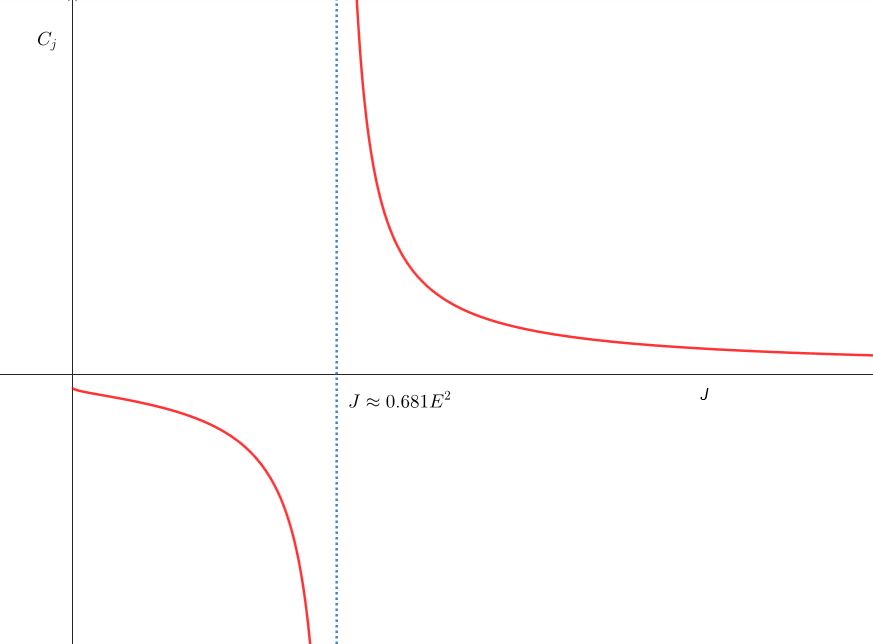
\includegraphics[scale=0.4]{immagini/kerr_heat_capacity.png}
    \caption{Calore specifico $C_J$ a $E=\cost$ per il buco nero di Kerr secondo eq. \ref{eq.calore_specifico_kerr}-\ref{eq.entropia_kerr_funzione_di_EJ}. Al valore $J=0$ si ottiene il risultato per Schwarzschild.}
    \label{fig.kerr_heat_capacity}
\end{figure}

Come noto dalla termodinamica, la trasformazione di Legendre permette di passare da un potenziale termodinamico ad un altro. L'energia libera di Gibbs è, per esempio:
\begin{equation}
    G(T, \Omega_H) = E - TS - \Omega_H J = \frac{1}{2}E
    \label{eq.en_libera_gibbs_ker}
\end{equation}
$G$ è continua alla discontinuità di $C_J$ e anche i suoi gradienti:
\begin{align*}
    \frac{\partial G}{\partial T}\Big|_{\Omega_H} && \frac{\partial G}{\partial \Omega_H}\Big|_T
\end{align*}
sono continui. Questo ci permette di dire che il fenomeno che avviene al valore critico $\frac{J^2}{E^4}\approx 0.464$ è una transizione di fase di II specie\footnote{Si ricorda che la transizione di fase di II specie implica la continuità di $G$ e delle sue derivate prima, ma la discontinuità delle seconde ovvero del calore specifico. Non c'è calore latente che invece contraddistingue le transizioni di I specie.}.
Si può fare un diagramma di fase (usando le espressioni delle derivate $\partial E/\partial S$ e $\partial E/\partial J$ prima calcolate):
\begin{equation}
    \frac{\Omega_H}{T} = \frac{\pi J}{S( \frac{1}{8\pi} - \frac{\pi J^2}{2S^2})}
    \label{eq.kerr_diagramma_fase}
\end{equation}
Se usiamo eq. \ref{eq.entropia_kerr_funzione_di_EJ} per esprimere $S$ e $J\approx 0.681E^2$, al valore critico si ha allora $\frac{\Omega_H}{T}\approx 5.843$. Il grafico di fase è mostrato in fig. \ref{fig.kerr_diagramma_fase}.
\begin{figure}
    \centering
    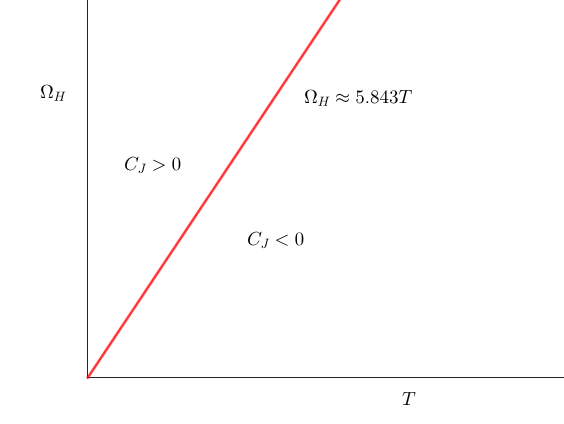
\includegraphics[scale=0.5]{immagini/kerr_diagramma_fase.png}
    \caption{Diagramma di fase per il buco nero di Kerr. In rosso il valore critico ottenuto da eq. \ref{eq.kerr_diagramma_fase} con $J\approx 0.681 E^2$.}
    \label{fig.kerr_diagramma_fase}
\end{figure}
La capacità termica $C_J$ ci permette di distinguere due differenti comportamenti del sistema:
\begin{itemize}
    \item $C_J < 0$: per un aumento di temperatura $\Delta T$, la massa del buco nero diminuisce e allora irradia di più, perdendo ancora più energia ecc.; il sistema è instabile e decade.
    \item $C_J > 0$: il buco nero può stare all'equilibrio termico con la radiazione.
\end{itemize}
\subsection{Termodinamica del buco nero di Schwarzschild-Tangherlini}
La soluzione di Schwarzschild-Tangherlini generalizza Schwarzschild ad una dimensione generica $d$ ed è descritta dalla metrica:
\begin{equation}
    ds^2 = - \left( 1 - \frac{\mu}{r^{d-3}}\right) dt^2 + \frac{dr^2}{1 - \frac{\mu}{r^{d-3}}} + r^2d\Omega_{d-2}^2
    \label{eq.schwarz_tangherlini}
\end{equation}
Con $d\Omega_{d-2}^2$ standard la metrica sulla $(d-2)$-sfera.

Per primo si calcola la temperatura di Hawking. Eseguiamo una rotazione di Wick $t \mapsto i\tau$:
\begin{equation*}
    ds^2 = \left( 1 - \frac{\mu}{r^{d-3}}\right) d\tau^2 + \frac{dr^2}{1 - \frac{\mu}{r^{d-3}}} + r^2d\Omega_{d-2}^2
\end{equation*}
La metrica è singolare in $r = \mu^{\frac{1}{d-3}} =: r_H$. Definiamo in analogia a quanto fatto per Schwarzschild:
\begin{equation*}
    \frac{x^2}{A} = r - r_H
\end{equation*}
con $A$ una costante opportuna da determinare. Segue che $dr = \frac{2x}{A}dx$.
Calcoliamo il termine che genera la singolarità nel limite $r \rightarrow r_H$:
\begin{align*}
    1 - \frac{\mu}{r^{d-3}} &= \left( 1 - \frac{\mu}{r^{d-3}}\right)\Big|_{r=r_H} + (d-3)\frac{\mu}{r^{d-2}}\Big|_{r=r_H}(r-r_H) + \dots \\
    &= (d-3)\frac{\mu}{\mu^{\frac{d-2}{d-3}}} + \dots= (d-3)\mu^{- \frac{1}{d-3}}\frac{x^2}{A} + \dots
\end{align*}
Chiamiamo per semplicità $B= (d-3)\mu^{- \frac{1}{d-3}} $. La metrica nel limite vicino alla singolarità è quindi:
\begin{align*}
    ds^2 &= \frac{B}{A^2}x^2d\tau^2 + \frac{4x^2}{A^2}\frac{A}{Bx^2}dx^2 + r_H^2d\Omega_{d-2}^2 \\
    &=\frac{B}{A^2}x^2d\tau^2 + \frac{4}{AB}dx^2 + r_H^2d\Omega_{d-2}^2
\end{align*}
A questo punto se scegliamo la costante iniziale come:
\begin{equation*}
    A = \frac{4}{B} = \frac{4}{(d-3)\mu^{-\frac{1}{d-3}}}
\end{equation*}
la metrica diventa:
\begin{equation*}
    ds^2 = \frac{B^2}{4}x^2d\tau^2 + dx^2 + M^2d\Omega_{d-2}^2 = \kappa^2 x^2 d\tau^2 + dx^2 + r_H^2d\Omega_{d-2}^2
\end{equation*}
che è un piano in $E_d$ in coordinate polari se identifichiamo $\tau \sim \tau + \frac{2\pi}{\kappa}$ così da non avere singolarità conica.  La temperatura è l'inverso del periodo del tempo euclideo quindi si trova:
\begin{equation}
    T = \frac{\kappa}{2\pi} = \frac{B}{4\pi} = \frac{(d-3)}{4\pi}\mu^{-\frac{1}{d-3}}
    \label{eq.temp_schwarz_tangherlini}
\end{equation}

Come passo successivo allo studio della termodinamica di questo buco nero, calcoliamo l'entropia di Bekenstein-Hawking secondo eq. \ref{eq.entropia_beken_hawking}. Serve calcolare l'area dell'orizzonte degli eventi: la metrica indotta sull'orizzonte è:
\begin{equation*}
    d\sigma^2 = r_H^2d\Omega_{d-2}^2 = r_H^2( \alpha_1 d\theta_1^2 + \alpha_2 d\theta_2^2 + \dots + \alpha_{d-2}d\theta_{d-2}^2)
\end{equation*}
con $\alpha_i(\bm\theta)$ i coefficienti che appaiono nella scrittura della metrica sulla $(d-2)$-sfera, funzioni dei vari angoli. Il determinante è pari a (osservando bene che $r_H$ è fattore comune a tutti i termini):
\begin{equation}
    \sigma = r_H^{2(d-2)}\prod_{i=1}^{d-2}\alpha_i(\bm\theta) = r_H^{2(d-2)}\det S^{d-2}
    \label{eq.sigma_indotta_scha_tang}
\end{equation}
L'area dell'orizzonte:
\begin{equation*}
    A = \int \sqrt{\sigma}d\Omega_{d-2} =  r_H^{d-2} \int\sqrt{\det S^{d-2}}d\theta_1\dots d\theta_{d-2} = r_{H}^{d-2}V(S^{d-2})
\end{equation*}
Se chiamiamo $V(S^{d-2})$ il volume della $(d-2)$-sfera. Quindi l'entropia:
\begin{equation}
    S = \frac{A}{4G} = \frac{r_H^{d-2}V(S^{d-2})}{4G} = \frac{V(S^{d-2})}{4G}\mu^{\frac{d-2}{d-3}}
    \label{eq.entropia_schwarz_tangherlini}
\end{equation}

Calcoliamo ora la massa di Komar associata al vettore di Killing $\xi = \partial_t$:
\begin{equation*}
    Q = \frac{c}{16\pi G} \oint_{\partial V} dS_{\mu\nu} \nabla^\mu \xi^\nu
\end{equation*}
con $c$ la costante da determinare e $dS_{\mu\nu}$ l'elemento di metrica indotta su $\partial V$, orientato. Consideriamo $\partial V$ come l'intersezione tra l'ipersuperficie $\Sigma$ dei tempi costanti e l'ipersuperficie $r= \textrm{cost.}$  Introduciamo il vettore normale di tipo tempo:
\begin{equation*}
    u = N^{-1}\partial_t \quad \textrm{ dove } \quad N = \sqrt{1 - \frac{\mu}{r^{d-3}}}
\end{equation*}
infatti $<u,u> = N^{-2} g_{tt} = -1$ e $< u, \partial_i> = 0$ per $i=1, \dots, d-2$.
Il vettore normale di tipo spazio possiamo definirlo come:
\begin{equation*}
    v = N\partial_r
\end{equation*}
che similmente a sopra soddisfa $<v,v> = 1$, $<v, \theta_i> = 0$ per $i= 1, \dots, d-2$. La misura indotta e orientata su $\partial V$ risulta:
\begin{equation*}
    dS^{\mu\nu} = (v^\mu u^\nu - u^\mu v^\nu)\sqrt{\sigma}d\theta_1\dots d\theta_{d-2}
\end{equation*}
con $\sigma$ di eq. \ref{eq.sigma_indotta_scha_tang}. Siccome vale in generale:
\begin{equation*}
    dS^{\mu\nu}\nabla_\mu\xi_\nu = \sqrt{\sigma}d\theta_1\dots d\theta_{d-2} ( - 2v^\nu u^\mu)\nabla_\mu \xi_\nu
\end{equation*}
 e $dS^{\mu\nu} = - dS^{\nu\mu}$, elaboriamo un attimo l'integrale di Komar ed eseguiamo i calcoli:
\begin{align*}
    Q &= \frac{c}{16\pi G}\oint_{\partial V} dS^{\sigma\rho}g_{\mu\sigma}g_{\nu\rho}g^{\alpha\mu}\nabla_\alpha \xi^\nu = - \frac{c}{16\pi G} \oint_{\partial V}dS^{\rho\sigma}\delta^\alpha_\sigma g_{\nu\rho}\nabla_\alpha \xi^\nu \\
     &=  \frac{c r^{d-2}}{8\pi G} \oint_{\partial V} v^\sigma u^\rho g_{\nu\rho}\nabla_\sigma \xi^\nu \sqrt{\det S^{d-2}}d\theta_1 \dots d\theta_{d-2} \\
    &=  \frac{c r^{d-2}}{8\pi G} \oint_{\partial V} v^r u^t g_{\nu r}\nabla_r \xi^\nu \sqrt{\det S^{d-2}}d\theta_1 \dots d\theta_{d-2} \\
    &= \frac{c r^{d-2}}{8\pi G} \oint_{\partial V} g_{\nu t}\nabla_r \xi^\nu \sqrt{\det S^{d-2}}d\theta_1 \dots d\theta_{d-2}
\end{align*}
Si deve solamente calcolare $\nabla_r \xi^t = \partial_r(\partial_t) + \tensor{\Gamma}{^t_{\lambda r}}\xi^\lambda = \tensor{\Gamma}{^t_{rt}}$. Il simbolo di Christoffel si determina da eq. \ref{eq.connlevicivita}:
\begin{equation*}
    \tensor{\Gamma}{^t_{rt}} = \frac{1}{2}g^{tt}g_{tt,r} = - \frac{1}{2}g^{tt}\partial_r\left( 1 - \frac{\mu}{r^{d-3}}\right) = - \frac{g^{tt}}{2}(d-3)\frac{\mu}{r^{d-2}}
\end{equation*}
allora:
\begin{equation*}
    Q = -\frac{c r^{d-2}}{16\pi G}\oint_{\partial V} g_{tt}g^{tt}(d-3)\frac{\mu}{r^{d-2}}\sqrt{\det S^{d-2}}d\theta_1 \dots d\theta_{d-2}
\end{equation*}
La massa (o energia, quantità conservata con il vettore di Killing $\partial_t$) è pertanto\footnote{Scelto $c=-1$. La definizione generale di questa quantità conservata pone come prefattore $-\frac{1}{8\pi G}$ che se usata qui fin dall'inizio ci farebbe ottenere un valore della massa/energia positivo.}:
\begin{equation}
    M = \frac{d-3}{16 \pi G} V(S^{d-2})\mu
    \label{eq.massa_schwarz_tangherlini}
\end{equation}
Si può verificare che eq. \ref{eq.temp_schwarz_tangherlini},
 \ref{eq.entropia_schwarz_tangherlini} e \ref{eq.massa_schwarz_tangherlini} soddisfano:
 \begin{equation*}
     dM = TdS
 \end{equation*}

 Da eq. \ref{eq.entropia_schwarz_tangherlini} possiamo esplicitare $\mu(S)$:
\begin{equation*}
     \mu(S) = (4S)^{\frac{d-3}{d-2}}\left( \frac{V(S^{d-2})}{G}\right)^{- \frac{d-3}{d-2}}
 \end{equation*}
così da sostituire in eq. \ref{eq.massa_schwarz_tangherlini} e ottenere:
\begin{equation}
    M(S) = \frac{d-3}{16\pi}\left( \frac{V(S^{d-2})}{G}\right)^{\frac{1}{d-2}}(4S)^{\frac{d-3}{d-2}}
    \label{eq.rel_fondam_massa_schwarz_tangh}
\end{equation}
oppure sostituendo in eq. \ref{eq.temp_schwarz_tangherlini}:
\begin{equation}
    T(S)= \frac{d-3}{4\pi}(4S)^{-\frac{1}{d-2}} \left( \frac{V(S^{d-2})}{G}\right)^{\frac{1}{d-2}}
    \label{eq.rel_fondam_temper_schwarz_tangh}
\end{equation}
Per eq. \ref{eq.rel_fondam_massa_schwarz_tangh} vale la relazione di Eulero:
\begin{equation*}
    M(\lambda S) = \lambda^{\frac{d-3}{d-2}}M(S)
\end{equation*}
Così possiamo calcolare, con l'obiettivo di ottenere la formula di Smarr:
\begin{align*}
    \frac{\partial M(\lambda S)}{\partial \lambda} &= S \frac{\partial M}{\partial(\lambda S)}= \frac{S}{\lambda}\frac{\partial M}{\partial S} =\frac{S(d-3)}{\lambda(d-2)}\left[\frac{d-3}{16\pi}\left(\frac{V(S^{d-2})}{G}\right)^{\frac{1}{d-2}}4^{\frac{d-3}{d-2}}S^{- \frac{1}{d-2}}\right] \\
    &= \frac{S(d-3)}{\lambda(d-2)}\left[\frac{d-3}{4\pi}\left(\frac{V(S^{d-2})}{G}\right)^{\frac{1}{d-2}}(4S)^{- \frac{1}{d-2}}\right] = \frac{S(d-3)}{\lambda(d-2)} T
\end{align*}
e anche:
\begin{equation*}
    \frac{\partial M(\lambda S)}{\partial \lambda} = \frac{\partial}{\partial \lambda}\left( \lambda^{\frac{d-3}{d-2}}\right)M(S) = \frac{d-3}{d-2}\lambda^{\frac{d-3}{d-2}-1}M(S)
\end{equation*}
Uguagliando queste due e mettendo poi $\lambda = 1$, si trova la formula di Smarr:
\begin{equation*}
    M(S) = TS
\end{equation*}

Possiamo ora calcolare la capacità termica e discuterne la stabilità. Se riarrangiamo eq. \ref{eq.temp_schwarz_tangherlini} per isolare $\mu(T)$:
\begin{equation*}
    \mu(T) = \left( \frac{d-3}{4\pi}V(S^{d-2})\right)^{d-3}T^{-(d-3)}
\end{equation*}
si ottiene sostituendo in eq. \ref{eq.massa_schwarz_tangherlini}:
\begin{equation*}
    M(T) = \frac{1}{4G}\left( \frac{d-3}{4\pi}V(S^{d-2})\right)^{d-2}T^{-(d-3)}
\end{equation*}
Dunque la capacità termica:
\begin{equation}
    C =  \frac{\partial M}{\partial T} = - \frac{d-3}{4G}\left( \frac{d-3}{4\pi}V(S^{d-2})\right)^{d-2}T^{-(d-2)} = - (d-3) \frac{M}{T^{d-2}} \label{eq.cap_termica_schwarz_tangh}
\end{equation}
Possiamo discuterne la stabilità:
\begin{itemize}
    \item $d=2$ allora $C = \frac{1}{4G}= \textrm{cost.}$ . Il buco nero può stare in equilibrio termico con la radiazione.
    \item $d= 3$ allora $C = 0$.
    \item $d > 3$ allora $C \propto - T^{-(d-2)}$. La capacità termica è sempre negativa con tendenza a zero per $T \rightarrow + \infty$. Non presenta estremi.  Il buco nero diventa più caldo quando irradia energia e pertanto decade in fretta sotto radiazione di Hawking.
\end{itemize}
Osserviamo che per $d=4$ si ottiene lo stesso risultato della capacità termica di Kerr con $J=0$.
\section{Buco nero di BTZ}
Consideriamo una gravità in 3-dim. con costante cosmologica $\Lambda < 0$. La teoria è descritta dall'azione:
\begin{equation*}
    I= \frac{1}{16\pi G} \int d^3x \sqrt{-g}( R - 2\Lambda )   
\end{equation*}
dove $\Lambda = - \frac{1}{l^2}$ e le equazioni del moto sono:
\begin{equation*}
    G_{\mu\nu} + \Lambda g_{\mu\nu} = 0
\end{equation*}
Come visto, uno spazio del genere è uno spazio di Einstein. Poiché siamo in dimensione 3, il tensore di Weyl è nullo, eq. \ref{eq.tensore_weyl}, e perciò lo spazio è anche a curvatura costante. Siccome uno spazio di Einstein a curvatura costante è di Minkowski, de Sitter o Anti-de Sitter, questa soluzione è \textbf{localmente $AdS_3$}.

La soluzione di \textbf{Banados-Teitelboim-Zanelli} \cite{btz} è descritta dalla metrica:
\begin{equation}
    ds^2 = - N^2dt^2 + \frac{dr^2}{N^2} + r^2(d\phi + N^\phi dt)^2
    \label{eq.metrica_btz}
\end{equation}
dove:
\begin{align*}
    N = \sqrt{-8GM + \frac{r^2}{l^2} + \frac{16 G^2 J^2}{r^2}} && N^\phi = - \frac{4GJ}{r^2}
\end{align*}
La metrica è singolare in $r= r_\pm$ definiti:
\begin{equation*}
    r_\pm^2 = 4GMl^2 \left[1 + \pm \sqrt{1 - \left(\frac{J}{Ml}\right)^2}\right]
\end{equation*}
Si deve avere $|J|\leq Ml$ così $r_+$ è l'orizzonte degli eventi e $r_-$ è quello di Cauchy. Per $|J| = Ml$ il buco nero è estremo e $r_+=r_-$.

Si dimostra che il buco nero di BTZ ha un'ergosfera al raggio:
\begin{equation}
    r_{erg}= (r_+^2 + r_-^2)^{1/2}
\end{equation}
corrispondente a richiedere $g_{tt} = 0$. Si dimostra che $r=r_+$ è un orizzonte di Killing per
\begin{equation*}
    \chi = \partial_v - N^\phi(r_+)d\Tilde{\phi}
\end{equation*}
dove $v, \Tilde{\phi}$ sono le coordinate di tipo Eddington-Finkelstein:
\begin{align*}
    dv = dt + \frac{dr}{N^2} && d\Tilde{\phi} = d\phi - \frac{N^\phi}{N^2}dr
\end{align*}
La gravità superficiale, calcolata da eq. \ref{eq.gravità_sup_quadrata}, risulta:
\begin{equation}
    \kappa = \frac{r_+^2 -r_-^2}{l^2r_+}
    \label{eq.grav_sup_btz}
\end{equation}
I valori $M, J$ sono massa e momento angolare come cariche associate ai vettori di Killing $\partial_t, \partial_\phi$ rispettivamente. Se si vuole eseguire il calcolo del loro integrale di Komar, bisogna considerare che diverge e serve pertanto sottrarre un background di $J=0$, $M=0$ rispettivamente.
L'entropia associata a questo buco nero è:
\begin{equation*}
    S = \frac{A_H}{4G} = \frac{2\pi r_+}{4G}
\end{equation*}

Il buco nero ha una rotazione. Gli osservatori localmente non rotanti hanno vettori tangenti:
\begin{equation*}
    \partial_t - N^\phi\partial_\phi
\end{equation*}
ovvero:
\begin{align*}
    <\partial_t - N^\phi\partial_\phi, \partial_\phi > &= 0 \\
    <\partial_t - N^\phi\partial_\phi, \partial_r > &= 0
\end{align*}
Questi però ruotano rispetto osservatori con vettori tangenti  $\partial_t$ ovvero degli osservatori localmente non rotanti a infinito o anche detti osservatori statici a infinito. La velocità angolare della rotazione è $\Omega = -N^\phi$ e pertanto la velocità di rotazione dell'orizzonte:
\begin{equation}
    \Omega_H = - N^\phi\Big|_{r=r_+} = \frac{4GJ}{r_+^2}
\end{equation}
Questo può essere mostrato considerando che gli osservatori localmente non rotanti sono tali che $\phi + N^\phi t = \cost$ lungo la linea di mondo\footnote{Questo deriva da $(\partial_t - N^\phi\partial_\phi)(\phi + N^\phi t) = 0$ con $\partial_t - N^\phi\partial_\phi$ che come detto è il loro vettore tangente alla linea di mondo.}. Dunque:
\begin{equation*}
    \phi = \cost - N^\phi t = \cost + \Omega t
\end{equation*}

La temperatura del buco nero può essere determinata dalla gravità superficiale di eq. \ref{eq.grav_sup_btz} in eq. \ref{eq.temperatura_hawking}. Si può esplicitamente fare il calcolo alternativo usando la sezione pseudoeuclidea, quindi facendo la rotazione di Wick $t = i\tau$:
\begin{equation*}
    ds_E^2= N^2d\tau^2 + \frac{dr^2}{N^2} + r^2(d\phi +iN^\phi d\tau)^2
\end{equation*}
Vicino a $r=r_+$ si ha lo sviluppo:
\begin{equation*}
    N^2 = N^2(r_+) + \frac{dN^2}{dr}\Big|_{r_+}(r-r_+) + o((r-r_+))
\end{equation*}
Facendo una semplice sostituzione $\rho^2 = r-r_+$, in questo limite:
\begin{equation*}
    ds_E^2 = \frac{4}{\frac{dN^2}{dr}\Big|_{r_+}}\left[ d\rho^2 + \left(\frac{dN^2}{dr}\Big|_{r_+}\right)^2\frac{\rho^2}{4} d\tau^2\right] + r_+^2(d\phi - i\Omega_H d\tau)^2
\end{equation*}
Quindi non si hanno singolarità coniche se $\tau \sim \tau + \frac{2\pi}{\frac{1}{2}\frac{dN^2}{dr}}\Big|_{r_+}$. Il calcolo della derivata è più semplice se usiamo la forma $N^2= \frac{1}{r^2l^2}(r^2-r_+^2)(r^2-r_-^2)$, così si ottiene la temperatura:
\begin{equation}
    T_H = \frac{r_+^2 - r_-^2}{2\pi l^2r_+}
    \label{eq.temp_btz}
\end{equation}
Nel caso di buco nero estremo, $r_+ = r_-$ e $T_H=0$.

La relazione fondamentale termodinamica:
\begin{equation}
    M(S,J) = \frac{G S^2}{2\pi^2l^2} + \frac{\pi^2 J^2}{2GS^2}
    \label{eq.rel_fondam_btz}
\end{equation}
fornisce correttamente $T = \frac{\partial M}{\partial S}$ e $\Omega_H = \frac{\partial M}{\partial J}$. La relazione di Eulero $M(\lambda S, \lambda^2 J)=\lambda^2 M(S,J)$ determina la formula di Smarr:
\begin{equation}
    M = \frac{1}{2}TS + \Omega_H J
    \label{eq.smarr_btz}
\end{equation}
Queste sono le proprietà generali termodinamiche del buco nero di BTZ.

Discutiamo ora la geometria globale del buco nero. Come già detto, questa soluzione è localmente $AdS_3$, quindi ogni intorno è isomorfo ad anti-de Sitter. Verrà mostrato come risultato finale che il buco nero BTZ è invece uno spazio quoziente di $AdS_3$\footnote{Lo spaziotempo massimale semplicemente connesso a curvatura costante negativa è lo spazio di ricoprimento universale $\Tilde{AdS}$ di anti-de Sitter. Per questo motivo scriveremo BTZ come spazio quoziente di $\Tilde{AdS}$  per un qualche gruppo di isometrie.}, corrispondente ad unire appropriatamente queste collezioni di intorni.
Tra le varie cose, questo vuol dire che la sua struttura a $r=\infty$ sia asintoticamente anti-de Sitter invece che asintoticamente piatta come avviene per Kerr.

Ricordiamo che $AdS_3$ è l'ipersuperficie di $\mathbb R^{2+2}$ definita da:
\begin{equation}
    X_1^2 + X_2^2 - T_1^2 -T_2^2 = -l^2
    \label{eq.ipersup_ads3}
\end{equation}
con metrica:
\begin{equation*}
    ds^2 = dX_1^2 + dX_2^2 - dT_1^2 - dT_2^2
\end{equation*}
e gruppo di isometrie $SO(2,2)$. La definizione dell'ipersuperficie può essere riassunta in forma di matrice con:
\begin{equation*}
    X = \frac{1}{l}\begin{pmatrix}
        T_1 + X_1 & T_2 + X_2 \\
        -T_2 + X_2 & T_1 - X_1
    \end{pmatrix}
\end{equation*}
così l'ipersuperficie eq. \ref{eq.ipersup_ads3} corrisponde a $\det X = 1$ e $X \in SL(2,\mathbb R)$.
Possiamo rappresentare le isometrie come gli elementi del gruppo:
\begin{equation*}
    SL(2,\mathbb R) \times \faktor{SL(2,\mathbb R)}{\mathbb Z_2} \approx SO(2,2)
\end{equation*}
Le due coppie di $SL(2,\mathbb R)$ agiscono come moltiplicazione destra e sinistra su un elemento $X$:
\begin{equation*}
    X \mapsto \rho_L X \rho_R
\end{equation*}
e vale inoltre $(\rho_L, \rho_R) = (-\rho_L, - \rho_R)$. Questo per quanto riguarda $AdS_3$.

Per $r \geq r_+$ parametrizziamo l'ipersuperficie eq. \ref{eq.ipersup_ads3} tramite:
\begin{align*}
    X_1 &= l\sqrt{\alpha}\sinh(\frac{r_+}{l}\phi - \frac{r_-}{l^2}t) \\
    X_2 &= l\sqrt{\alpha - 1}\cosh( \frac{r_+}{l^2}t - \frac{r_-}{l}\phi) \\
    T_1 &= l\sqrt{\alpha}\cosh(\frac{r_+}{l}\phi - \frac{r_-}{l^2}t)\\
    T_2 &= l\sqrt{\alpha - 1} \sinh(\frac{r_+}{l^2}t - \frac{r_-}{l}\phi)
\end{align*}
dove $\phi, t \in \mathbb R$ su $AdS_3$ e 
\begin{equation*}
    \alpha = \frac{r^2 - r_-^2}{r_+^2 - r_-^2}
\end{equation*}
Con questa parametrizzazione possiamo ricondurci alla regione $r\geq r_+ $ di BTZ se però identifichiamo $\phi \textrm{ mod } 2\pi$ . La metrica indotta coincide con quella di BTZ. Per le altre regioni di BTZ servono differenti parametrizzazioni (vedi \cite{btz}), corrispondenti ad altre zone del diagramma di Penrose.

Questa identificazione di $\phi$ con $\phi \textrm{ mod } 2\pi$ è un'isometria di $AdS_3$ (è un boost nei piani $X_1$-$T_1$ e $X_2$-$T_2$) a cui corrispondono gli elementi di $(\rho_L, \rho_R)$ con:
\begin{equation*}
    \rho_L = \begin{pmatrix}
        e^{\pi(r_+-r_-)/l} & 0 \\
        0 & e^{-\pi(r_+-r_-)/l}
    \end{pmatrix}
\end{equation*}
\begin{equation*}
    \rho_R = \begin{pmatrix}
        e^{\pi(r_+ + r_-)/l} & 0 \\
        0 & e^{-\pi(r_+ + r_-)/l}
    \end{pmatrix}
\end{equation*}
SI può quindi mostrare che:
\begin{equation*}
    BTZ = \faktor{AdS_3}{<(\rho_L,\rho_R)>}
\end{equation*}
dove $<(\rho_L,\rho_R)>$ è il gruppo discreto generato dagli elementi $(\rho_L,\rho_R)$.

Questo risultato è importante in quanto $AdS_3$ è una varietà estremamente semplice e virtualmente priva di struttura; tuttavia con le opportune identificazioni, si può convertire in uno spaziotempo (BTZ) con proprietà molto simili a Kerr $(3+1)$-dimensionale. In tutto ciò BTZ rimane uno spaziotempo a curvatura costante e inoltre, come verrà visto in \S\ref{para.chern}, la gravità 3-dimensionale è esprimibile come una teoria di gauge che può essere quantizzata.